\documentclass[10pt, twocolumn]{article}

%math
\usepackage{amsmath}
\usepackage{amssymb}
\usepackage{mathtools}
%logic
\usepackage{pgffor}
\usepackage{ifthen}
%science
\usepackage[separate-uncertainty=true]{siunitx}
\usepackage[version=4]{mhchem}
%language
\usepackage[english]{babel}
%formatting
\usepackage[a4paper, portrait, margin=1in]{geometry}
\usepackage{cuted}
\usepackage[small]{titlesec}
\usepackage[hidelinks]{hyperref}
\usepackage{parskip}
%images and plots
\usepackage{graphicx}
\usepackage[justification=centering]{caption}
\usepackage{subcaption}
\usepackage{float}
\usepackage{pgf}
\usepackage{import}
%tables
\usepackage{booktabs}
\usepackage{makecell}
%citation, quatation and lists
\usepackage[style=numeric,maxcitenames=2,sorting=none,doi=false,
url=false,isbn=false,eprint=false]{biblatex}
\usepackage[noabbrev,nameinlink]{cleveref}
\usepackage{csquotes}
\usepackage[nottoc]{tocbibind}
\usepackage{acro}


%setup plugins
\addbibresource{literature.bib}
\captionsetup{justification=centering}
\hypersetup{colorlinks=true,linkcolor=blue}

\DeclareSIUnit\angstrom{\text {Å}}
\DeclareSIUnit\bar{bar}
\sisetup{
	range-phrase = { to }
}

% Custom \citeauthoryear command with hyperref -> Rost et al. (2019) 
\DeclareCiteCommand{\citeauthoryear}
{\boolfalse{citetracker}%
\boolfalse{pagetracker}%
\usebibmacro{prenote}}
{\ifciteindex
{\indexnames{labelname}\indexfield{year}}
{}%
\printtext[bibhyperref]{%
    \printnames{labelname}%
    \setunit{\addspace}%
    \printtext{(}%
    \printfield{year}%
    \printtext{)}}}
{\multicitedelim}
{\usebibmacro{postnote}}

%  setup custom commands
\newcommand{\imcite}[2][]{From \cite[#1]{#2}.}
\newcommand{\imcitetwo}[2][]{Based on \cite[#1]{#2}.}
\newcommand{\integral}[4]{\int_{#1}^{#2} #3 \mathrm{d} #4}
\newcommand{\derivative}[2]{\frac{\mathrm{d}}{\mathrm{d} #1} #2}

%set up acronyms
\DeclareAcronym{sem}{
  short=SEM,
  long=scanning electron microscope,
}
\DeclareAcronym{pe}{
	short=PE,
	long=primary electrons
}
\DeclareAcronym{se}{
	short=SE,
	long=secondary electrons
}
\DeclareAcronym{be}{
	short=BE,
	long=backscattered electrons
}
\DeclareAcronym{edx}{
	short=edx,
	long=energy-dispersive X-ray spectroscopy
}

% Document
\begin{document}
\pagenumbering{arabic}
\begin{strip}
	\begin{centering}
	\huge Semiconductor Physics Laboratory \RN{1}\\
	\LARGE A2: Scanning electron microscopy \\
	\vspace{0.35cm}
	\normalsize Simon Legtenborg, 3773994 \\ 
	\normalsize Experiment conducted on 22.11.2024 \\
	\vspace{1cm}
\end{centering}

\end{strip}
\paragraph{Abstract}
This lab report explores various applications of a scanning electron
microscope.
Using secondary electron detection, the topography of an unknown
semiconductor sample is analyzed.
Additionally, material characteristics are determined through
X-ray emission and backscattered electrons.

\section{Electron Matter Interactions}
To understand the working principle of a \ac{sem}, it is necessary to consider the
interaction between electrons and solid matter.
For that, one observes the path of an electron which is emitted directly from the cathode
and head to the sample. Those electrons are called \textit{\ac{pe}}.
After arriving at the surface, the electrons undergo elastic and inelastic scattering.
Due to complex interactions between \ac{pe} and the atoms
inside the sample, multiple interaction products are generated, which can
be classified into different categories.
The categories, that are relevant for conducing the experiment are the
following:
\begin{itemize}
	\item Secondary electrons
	\item Backscattered electrons
	\item X-Ray emission
\end{itemize}
After arriving at the surface, the electrons spread due to
small-angle scattering in a pear shaped area around the collision point.
Different interactions are located at different spatial regions.
This is visualized in \cref{fig:birne}.
The higher the atomic number, the stronger is the scattering of the
electrons.
\subsection{Secondary Electrons}
\ac{pe} collide with the bounded electrons and ionize the
corresponding atoms.
Those now free electrons from the top layer can diffuse out of the
material and are called \ac{se}.
Due to the high energy loss during ionization, \ac{se}
have a low kinetic energy compared to \ac{pe}.
The energy distribution is shown in \cref{fig:electrons}.
To quantify the relation between \ac{pe} and \ac{se}, one
uses the electron yield $\delta_\mathrm{SE} = \text{\# SE} / \text{\# PE}$.
In the typical case of \ac{pe} with energies between
\qtyrange{10}{25}{\kilo\electronvolt}, $\delta_\text{SE}$ is far below one.
It is possible to get a topographic contrast from \ac{pe}.
The electron yield is strongly dependent on the angle of incidence of
the surface with $\delta_\mathrm{SE} \simeq \cos(\theta)$.
If there is a change in height, there must also be a change of the
incidence angle $\theta$ which alters the image.
Note, that only height changes and not the absolute height defines the
topography contrast.
Due to the fact, that the absorption length for secondary electrons is
only a couple nanometers thin, this method delivers precise information
about a local structure.
\begin{figure}[H]
	\centering
	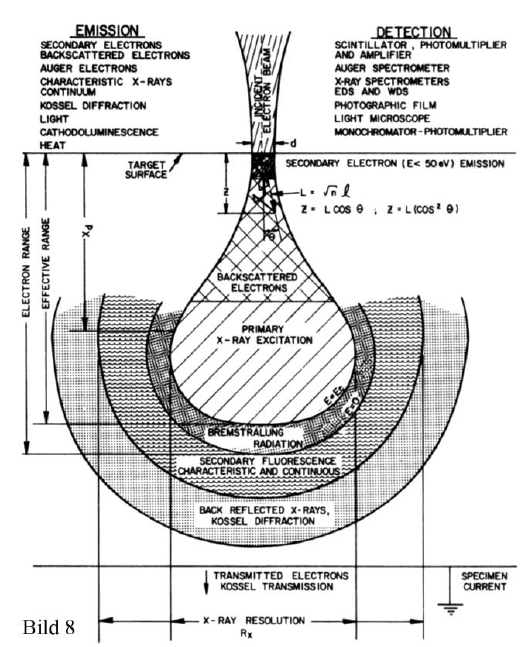
\includegraphics[width=0.95\linewidth]{../assets/birne.png}
	\caption{Interaction area of electrons. \imcite{rem_script}}
	\label{fig:birne}
\end{figure}
\ac{se} are caught by the detector and converted into
an electrical signal.
The scanning electron microscope uses a light-sensitive photo multiplier
with a scintillator disc and a metal grid for collecting electrons.
The metal grid and the scintillator disk can be biased to filter
electrons with different energies.
For \ac{se}, the metal grid is positively charged to attract electrons
from a larger spatial region.
After the electrons collide with the scintillator, the material emits
light, which can be detected by the photo multiplier.
The more electrons collide with the scintillator, the higher is the
intensity of the emitted light and the stronger is the
electrical signal which leads to a brighter pixel on the image.

Not only the surface topography can affect the electron yield but also
the electrical surface potentials.
\begin{figure}[H]
	\centering
	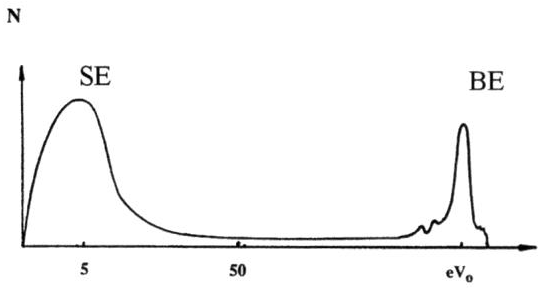
\includegraphics[width=0.95\linewidth]{../assets/elektronen.png}
	\caption{Electron yield as a function of energy. \imcite{rem_script}}
	\label{fig:electrons}
\end{figure}

\subsection{Backscattered Electrons}
A large proportion of \ac{pe} won't ionize the material but
rather be reflected or backscattered by the nuclei of the sample.
Due to the heavy nucleus, the electrons will primarily change their
direction.
These electrons are called \ac{be}. In a physical sense, \ac{be} can't be
distinguished from \ac{se}, but their kinetic energy is much higher
which provides a good indicator.
This leads to the definition that electrons with energies in the order
of magnitude of $\mathrm{e} V_0$, where $\mathrm{e}$ is the elementary
charge and $V_0$ the potential difference of the cathode, are
categorized as \ac{be}.

The electron yield for backscattered electrons is very dependent on
the atomic number $Z$ with $\delta_\text{BS} = \# BS / \# PE
	\propto \sqrt{Z}$.
Because of this dependency and the fact, that \ac{be}
contrast is less affected by surface layers and local surface fields,
they offer a reliable
method to detect material contrast.
This is visualized in \cref{fig:material_contrast}.

To detect \ac{be}, one can use a solid-state p-n
junctions with multiple sectors.
Those detectors are reverse biased to establish an electric field which
can collect and count the arriving electrons.
A stronger signal corresponds to a higher number of collected electrons.
\begin{figure}[H]
	\centering
	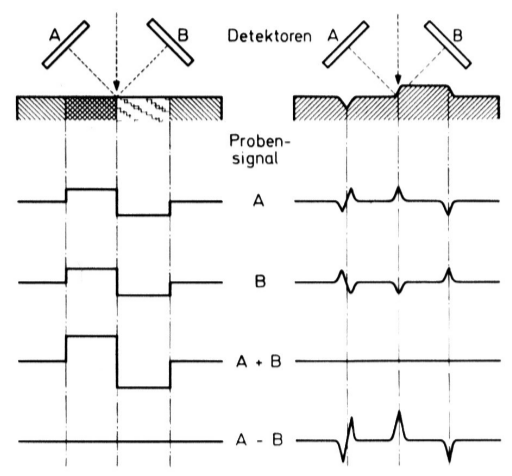
\includegraphics[width=0.95\linewidth]{../assets/material.png}
	\caption{Material contrast (left) and topographical contrast (right) detection.
		\imcite{rem_script}}
	\label{fig:material_contrast}
\end{figure}

\subsection{X-ray Emission}
The X-ray spectrumlconsists of two parts.
The first part consists of bremsstrahlung, which is generated during the
deceleration of the electrons.
This type of radiation is, due to it's origin, observable in every X-ray
emission experiment and cannot be used to identify materials.

For that, there exists the second part, which is called characteristic
radiation.
During ionization, electrons from energetically higher states relax
into a more favorable states.
The resulting energy differnce generates an X-ray photon.
Due to the  discrete energies of the electron states,
the resulting energy-intensity spectra will contain sharp, well-defined
peaks, which are characteristic for every material.
The energy transitions $K_{\mathrm{\alpha}_{1}}$ and
$K_{\mathrm{\alpha}_{2}}$ are primarely observed.

To analyse X-ray radiation, one can conduct an energy dispersive
spectrometer experiment.
A cooled silicium diode detector is driven reverse biased to create an
electric field.
If an X-ray photon enters the material, it will create electron-hole-pairs
which can be separated and counted.
The higher the number of electrons, the higher the energy of the X-ray
photon.
By analyzing the positions of the peaks in the spectrum, qualitative
conclusings about the compositions can be drawn.
Through the corresponding intensity, quantitiative conclusions are also
possible.

\section{Measurement Methods}

\subsection{\ac{sem} Setup}
\begin{figure}
	\centering
	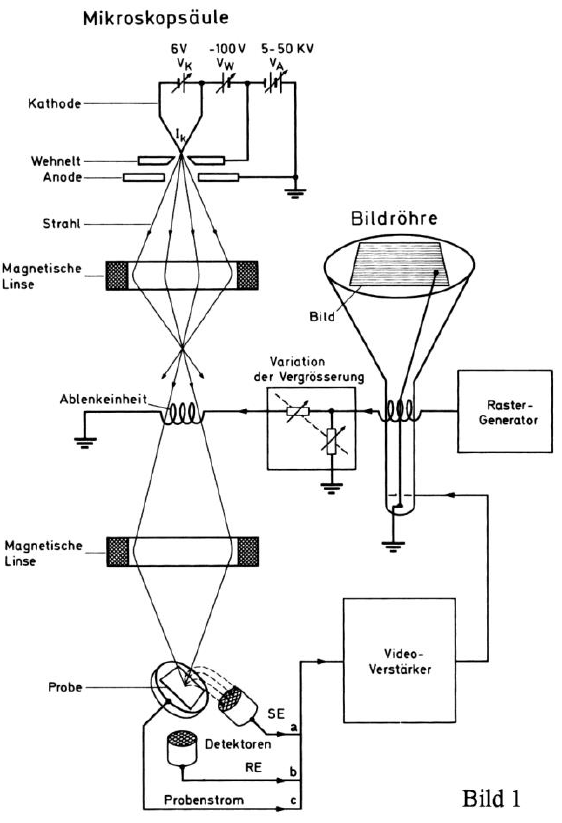
\includegraphics[width=0.95\linewidth]{../assets/aufbau.png}
	\caption{Setup of a scanning electron microscope. \imcite{rem_script}}
	\label{fig:general_structure}
\end{figure}
A schematic	representation of a scanning electron microscope is shown in
\cref{fig:general_structure}.
A cathode emits electrons that are accelerated afterwards by an anode
and focused into a nanometer-wide beam by multiple magnetic lenses.

A goal of a \ac{sem} is to probe the sample at different spots.
To achieve this, one can use the magnetic field of a coil that deflects
the electron beam.
As a result, the electron beam scans across the surface in a raster
pattern. Various detectors are positioned near the sample to measure
different interaction products resulting from the electrons colliding
with the sample atoms. This allows for the generation of an intensity
signal that depends on the position of the electron beam.

For older devices, the electron beam position is synchronized
with a CRT.
In newer devices, the signal is digitized and can be outputted in
various formats.

\subsection{Electron Beam Generation}
Electrons can be produced via thermionic emission, such as with a tungsten hairpin cathode that is used in this experiment.
The cathode is heated to a temperature range of
\qtyrange{2600}{3000}{\kelvin} to overcome the work function of
\qty{2.5}{\electronvolt} through thermal excitation.
The cathode is surrounded by a Wehnelt-cylinder, on which a voltage is
applied.
The cylinder is used as a first focusing mechanism.
This is visualized in \cref{fig:wolfram}.
\begin{figure}
	\centering
	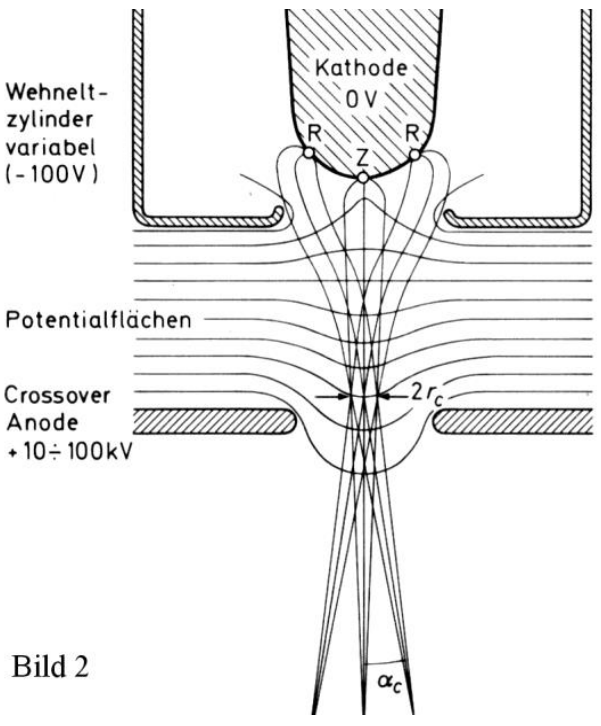
\includegraphics[width=0.95\linewidth]{../assets/wolfram.png}
	\caption{Geometric arrangement of the cathode and the Wehnelt-cylinder.
		\imcite{rem_script}}
	\label{fig:wolfram}
\end{figure}
There also exist \ce{LaB6} cathodes, which consist of a small rod-shaped
lanthanum hexaboride single crystal.
This crystal is indirectly heated to temperature ranging
from \qtyrange{1700}{2100}{\kelvin}.
Due to the lower work function of \qty{2.7}{\electronvolt} the cathode
can work at a lower temperature.

Apart from thermionic emission, there also exist field emission, where
the quantum mechanical tunneling effect is utilized to generate electrons.
This provides a more precise beam but is also more complex to operate.

\subsection{Electron Lenses}
After being emitted by the cathode, the electron beam cross-section
needs to be reduced further.
To achieve this, electron lenses are used.
The most common architecture is a magnetic coil that generates a
rotationally symmetric field.
The field amplitude is gaussian-shaped along the symmetry axis.
When electrons arrive at the coil, they are forced to move in a helix
trajectory and merged into the focal point.

As with optical lenses, electron lenses show a variety of
aberrations, which need to be considered.
\begin{itemize}
	\item \textit{Spherical aberration} occurs because off-axis electrons
	      are deflected more strongly than on-axis electrons, resulting in a
	      shorter focal point. Spherical aberration increases at large
	      aperture angles.
	\item \textit{Axial astigmatism} is an imaging error related to the
	      magnetic inhomogenities, that leads to a deviation from rotational
	      symmetry.
	      This deviation causes different focal points for different beam
	      planes.
	\item \textit{Chromatic errors} are another type of aberration
	      which originates from the velocity distribution of the electrons.
	      Different velocities result in different wavelengths and different
	      focal points.
	\item \textit{Diffraction errors} occur because of the small aperture
	      angle and the resulting single slit interference of electron waves.
	      This leads to a blurred lens focus.
	      As diffraction errors increase with small aperture angles and
	      spherical aberrations increase with large angles, one can find an
	      optimal angle that minimizes the total error.
\end{itemize}

\section{Results and Discussion}
\subsection{Hall Effect Measurements at Room Temperature}
Measurements were performed on p-type silicon (\ce{p-Si}, $d=\qty{500}{\micro\meter}$), 
zinc oxide (\ce{ZnO}, $d=\qty{1}{\micro\meter}$), zinc tin oxide (\ce{ZTO}, 
$d=\qty{1.3}{\micro\meter}$) and copper iodide (\ce{CuI}, $d=\qty{0.339}{\micro\meter}$) 
thin film samples.
Using the Van der Pauw method, the resistivity, Hall carrier concentration and Hall 
coefficients were determined for each sample.

With four distinct sample contact configurations, four measurements were performed 
per sample. 
The resistivity $\rho$ was calculated using \cref{eq:hall_resistivity}, 
the Hall coefficient $R_{\mathrm{H}}$ using \cref{eq:hall_coefficient_van_der_pauw},
the carrier concentration $n$ using \cref{eq:hall_concentration} 
and the Hall mobility $\mu_{\mathrm{H}}$ using \cref{eq:hall_mobility}.
The results are averaged in \cref{tab:hall_results_detail}, 

An important observation is the varying sign of $R_{\mathrm{H}}$. 
Since the sign of the Hall coefficient is determined by the majority charge carrier
(positive for holes, negative for electrons), this indicates that holes are the majority
charge carrier for \ce{p-Si} and \ce{CuI}. 
Electrons are the majority charge carrier for \ce{ZnO} and \ce{ZTO}. 

\subsection{Temperature Dependent Hall Effect Measurements}
Temperature dependent Hall effect measurements for a bulk \ce{ZnO} sample 
were performed in the Temperature range from \qty{20}{\kelvin} to \qty{325}{\kelvin}.
Both the Hall mobility and Hall carrier concentration were determined for each 
temperature and are displayed in 
\cref{fig:zno_hall_effect_n,fig:zno_hall_effect_mu} respectively.

The graph of the Hall carrier concentration in \cref{fig:zno_hall_effect_n} shows a 
linear decrease with increasing inverse temperature. 
This observation can be explained using the low temperature approximation 
\cref{eq:n_T_approx_low}:

\begin{align}
	&n = \text{const.} \cdot T^{3/2} \exp\left( \frac{-E_{\mathrm{D}}^{b}}{2 \mathrm{k}T} \right) \\
	\ln(&n T^{-3/2}) = \ln(\text{const.}) - \frac{E_{\mathrm{D}}^{b}}{2 \mathrm{k}} \cdot \frac{1}{T} 
	\label{eq:n_T_approx_low_linear}
\end{align}

Using a linear fit, one obtains a slope of \qty{\taskTwoSlope}{\kelvin}.
With \cref{eq:n_T_approx_low_linear}, this slope can be used to determine the donor energy 
$E_{\mathrm{D}}^{b} = \qty{\taskTwoEnergy}{\milli \electronvolt}$.
For high temperatures, the carrier concentration saturates, since all donors are ionized.
By applying \cref{eq:n_T_approx_high}, the donor concentration can be estimated to be
$N_{\mathrm{D}} = \qty{\taskTwoND}{\per \meter\cubed}$.

The Hall mobility in \cref{fig:zno_hall_effect_mu} can be parted into three distinct 
regions.
For every region, the data follows a linear trend, that can be described using three 
linear fits.
The first region has a slope of \num{\taskTwoSlopeOne}, the second region has a slope of
\num{\taskTwoSlopeTwo} 
and the third region has a slope of \num{\taskTwoSlopeThree}.

In a $\log-\log$ plot, a linear function indicates a power law relationship, whereby the
slope of the line corresponds to the exponent of the power law. 
Since the mobility is determined by scattering processes, that have a characteristic 
temperature dependence, different scattering mechanisms can be identified. 
The first region, where $\mu_\mathrm{H} \propto T^{3 / 2}$, can be explained by 
ionized impurity scattering.
The second region, where $\mu_\mathrm{H} \propto T^{\taskTwoSlopeTwo} \simeq T^{-1/2}$, 
can be explained by piezoelectric potential scattering.
The third region, where $\mu_\mathrm{H} \propto T^{\taskTwoSlopeThree} 
\simeq T^{-3 / 2}$, can be explained by deformation potential scattering.

\begin{figure*}
	\centering
	\begin{subfigure}{0.48\textwidth}
		\centering
		\includegraphics{../plots/task_2_n.pdf}
		\caption{Hall carrier concentration of a bulk \ce{ZnO} sample as a function of temperature.}
		\label{fig:zno_hall_effect_n}
	\end{subfigure}
	\hfill
	\begin{subfigure}{0.48\textwidth}
		\centering
		\includegraphics{../plots/task_2_mu.pdf}
		\caption{Hall mobility of a bulk \ce{ZnO} sample as a function of temperature.}
		\label{fig:zno_hall_effect_mu}
	\end{subfigure}
	\caption{Temperature-dependent Hall effect measurements of a bulk \ce{ZnO} sample.}
	\label{fig:zno_hall_effect_combined}
\end{figure*}

\subsection{Interpretation of an Unusual Data Set}
Temperature dependent Hall effect measurements of a \ce{ZnO} thin film sample
were performed in the temperature range from \qty{20}{\kelvin} to \qty{325}{\kelvin}.
However, the dataset does not seem to match a single donor model, as the carrier 
concentration, see \cref{zno_hall_n} raises with falling temperature.
The uncorrected data is shown in \cref{zno_hall_n}, it does not show a linear trend. 

This could indicate that the sample is not a single donor system. 
However, \citeauthoryear{look} suggest, that the sample is a single donor system, 
but a two-layer Hall analysis needs to be performed to correct the data. 
Since \ce{ZnO} and sapphire have a large lattice mismatch, a highly dislocated region 
at the interface between thin film and substrate is generated during growth. 
This high-density region of stacking faults significantly affects the carrier 
concentration as well as the mobility as a function of temperature and does not
show a linear trend.

For a two-layer Hall analysis, we index the \ce{ZnO} thin film as '\num{1}' and the 
dislocated region at the interface as index '\num{2}'. 
Using \cref{eq:multilayer_sum_1,eq:multilayer_sum_2} we can find the following identities
\begin{align}
	\sigma_{\square}=e\mu_{\mathrm{H}1}n_{ \square 1}
	+e \mu_{\mathrm{H}2} n_{ \square 2} \\
	R_{\square} \sigma_{\square}^{2}=e \mu_{\mathrm{H} 1}^{2} n_{ \square 1} 
	+ e\mu_{\mathrm{H} 2}^{2} n_{ \square 2}
\end{align}
It is possible to find an analytical expression for 
$\mu_\mathrm{H}$ and $n$:
\begin{align}
	\mu_{\mathrm{H}}&=R_{\square} \sigma_{\square}
	=\frac{R_{\square} \sigma_{\square}^{2} /d}{\sigma_{\square} / d} \\
	&=\frac{\mu_{\mathrm{H}1}^{2}n_{1}
	+\mu_\mathrm{H2}^{2} n_{\square2} /d}{\mu_{\mathrm{H}1}n_{1}
	+\mu_{\mathrm{H}2}n_{\square{2}} /d} \\
	n_{}=\frac{n_{ \square}}{d}&=\frac{1}{eR_{\square}d}
	= \frac{\sigma^{2}_{\square}/ d^{2}}{eR_{\square}\sigma_{\square}^{2} / d}  \\
	&=\frac{(\mu_{\mathrm{H}1}n_{1}
	+\mu_{\mathrm{H}2}n_{\square2} /d)^{2}}{\mu_{\mathrm{H}1}^{2}n_{1}
	+\mu_{\mathrm{H}2}^{2} n_{ \square 2} /d}
\end{align}
Since the donor atoms freeze at low temperatures, the interface layer must be dominant 
in this region. 
Since the paper suggest that the layer's carrier concentration and mobility is 
temperature independent, we can approximate
$n_{}=n_{ \square 2} / d = \qty{\taskThreeInterfaceN}{\per\meter\cubed}$ 
and 
$\mu_{\mathrm{H}}=\mu_{\mathrm{H 2}} = \qty{\taskThreeInterfaceM}{\centi\meter\squared\per\volt\per\second}$
for $T \to \qty{0}{\kelvin}$. 

An expression for the corrected hall mobility $\mu_{\mathrm{H} 1}$ and  
hall carrier concentration $n_{1}$ can now 
be found:
\begin{align}
	\mu_{\mathrm{H} 1}=\frac{\mu_{\mathrm{H}}^{2} n_{}- \mu_{2} ^{2} 
	n_{ \square 2} /d}{\mu_{\mathrm{H}} n_{} - \mu_{2} n_{\square 2} / d} \\
	n_{1} = \frac{(\mu_{\mathrm{H}}n_{}-\mu_{2}n_{\square 2} 
	/ d)^{2}}{\mu_{\mathrm{H}}^{2}n_{}-\mu_{2}^{2} n_{\square 2} / d}	
\end{align}
The corrected carrier density is also displayed in \cref{zno_hall_n} and can
now be identified with the single-donor case.
Using linear regression, a slope of \num{\taskThreeSlope} and a corresponding donor 
energy of $\qty{\taskThreeEnergy}{\milli \electronvolt}$ can be determined.
The donor concentration can be estimated using \cref{eq:n_T_approx_high} to be
$N_{\mathrm{D}} = \qty{\taskThreeND}{\per\meter \cubed}$

The corrected mobility is displayed in \cref{zno_hall_mu} and shows a linear trend with a 
slope of \num{\taskThreeMobilityOne} for the first region and a slope of 
\num{\taskThreeMobilityThree} for the second region.
The log-log plot indicates a power law relationship, that can be explained by
deformation potential scattering since 
$\mu_\mathrm{H} \propto T^{\taskThreeMobilityThree} \simeq T^{-3/2}$.

\begin{figure*}
	\centering
	\begin{subfigure}[t]{0.48\textwidth}
		\centering
		\includegraphics{../plots/task_3_n.pdf}
		\caption{Corrected and uncorrected Hall carrier concentration of a \ce{ZnO} thin 
		film sample as a function of temperature.}
		\label{zno_hall_n}
	\end{subfigure}
	\hfill
	\begin{subfigure}[t]{0.48\textwidth}
		\centering
		\includegraphics{../plots/task_3_mu.pdf}
		\caption{Corrected and uncorrected Hall mobility of a \ce{ZnO} thin film sample as 
		a function of temperature.}
		\label{zno_hall_mu}
	\end{subfigure}
	\caption{Corrected and uncorrected Hall effect measurements of a \ce{ZnO} thin film sample.}
	\label{fig:zno_hall_effect_corrected}
\end{figure*}

\begin{table*}
\centering
\input{../plots/resistivity_hall.tex}
\caption{Hall effect quantities of p-Si, ZnO, ZTO and CUI thin film samples.}
\label{tab:hall_results_detail}
\end{table*}

\clearpage
\begin{strip}
	\printbibliography[heading=bibintoc]
	\listoffigures
	\listoftables
\end{strip}
$\phantom{=}$
\end{document}
